\documentclass[10pt,a4paper]{report}
\usepackage[utf8]{inputenc}
\usepackage[T1]{fontenc}
\usepackage{amsmath}
\usepackage{amssymb}
\usepackage{graphicx}
\usepackage{ragged2e}
\usepackage{multicol}
\usepackage[margin=1cm]{geometry}
\usepackage{nopageno}
\usepackage{hyperref}
\graphicspath{ {./images/} }
\begin{document}
	\LARGE \noindent \justifying \textbf{Application title:} \par
	\noindent 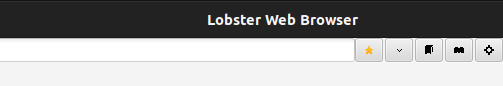
\includegraphics[width=80mm]{images/title.png} \par
	\normalsize \justifying \noindent The app has a title: Lobster Web Browser. \par
	
	
	\LARGE \noindent \justifying \textbf{Application icon:} \par
	\noindent 
\includegraphics[width=50mm]{images/icon.png} \par
	\normalsize \noindent The app has an icon (see above). \par
	
	
	\LARGE \noindent \justifying \textbf{Tabs:} \par
	\noindent 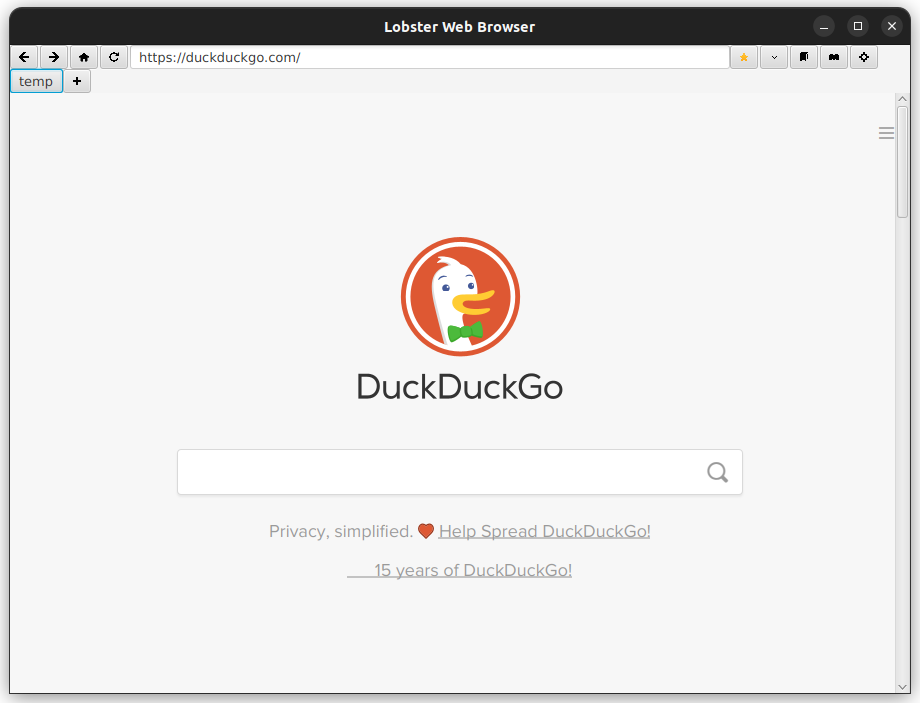
\includegraphics[width=80mm]{images/tabs.png} \par
	\normalsize \noindent By clicking on a “Temp” button, it will change tab to the respective tab. Each tab has its own webview. Tabs can be deleted by mouse wheel clicking on the “Temp” button for that tab. Internally, the current tab is stored in an object called a TabStorer which allows for the current tab to be updated and for every functionality to “see” this update. If there is only one tab and this tab is deleted, a new tab will be created to replace the deleted one. New tabs start on the homepage, which is duckduckgo by default. \par
	
	
	\LARGE \noindent \justifying \textbf{Tab context menu:} \par
	\noindent 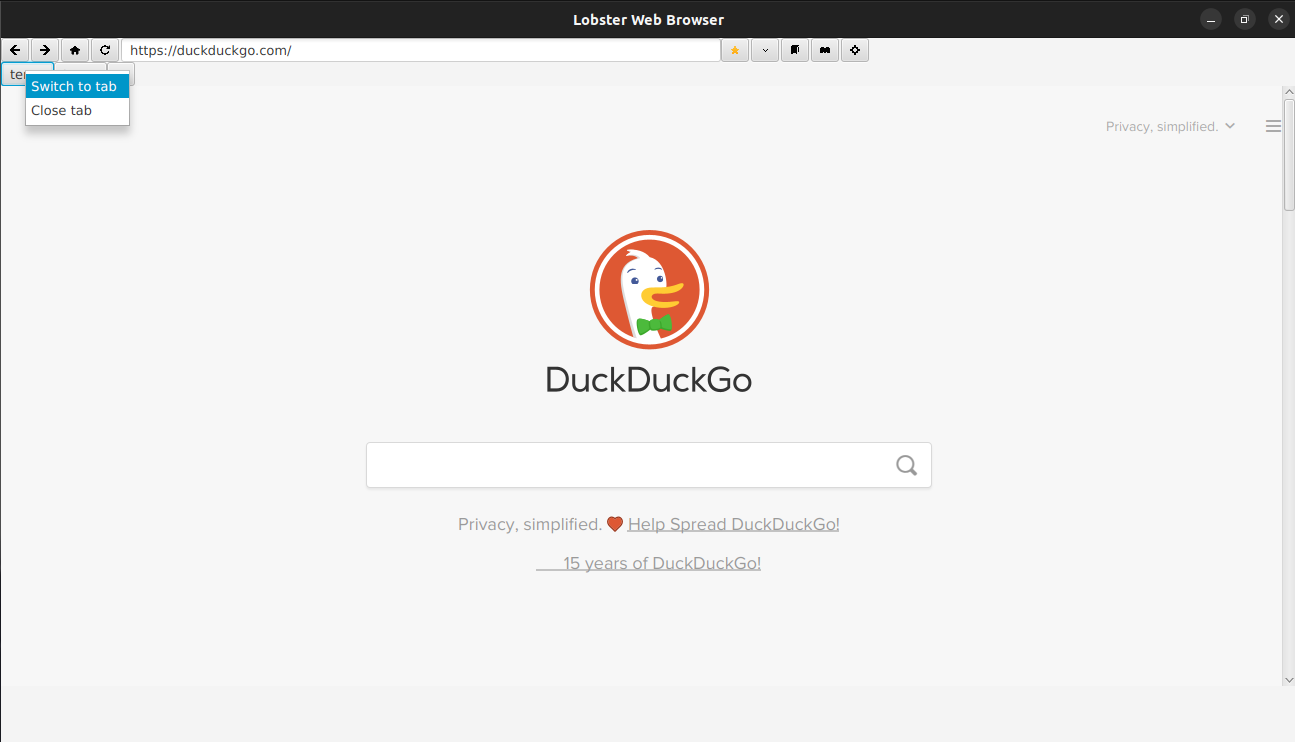
\includegraphics[width=80mm]{images/tabContextMenu.png} \par
	\normalsize \noindent Right Clicking on a tab brings up a context menu with two options: Close tab and Switch to tab. Clicking on one of these options will close or delete the tab (depending on the option selected). \par
	
	\pagebreak
	
	\LARGE \noindent \justifying \textbf{Add tab:} \par
	\noindent 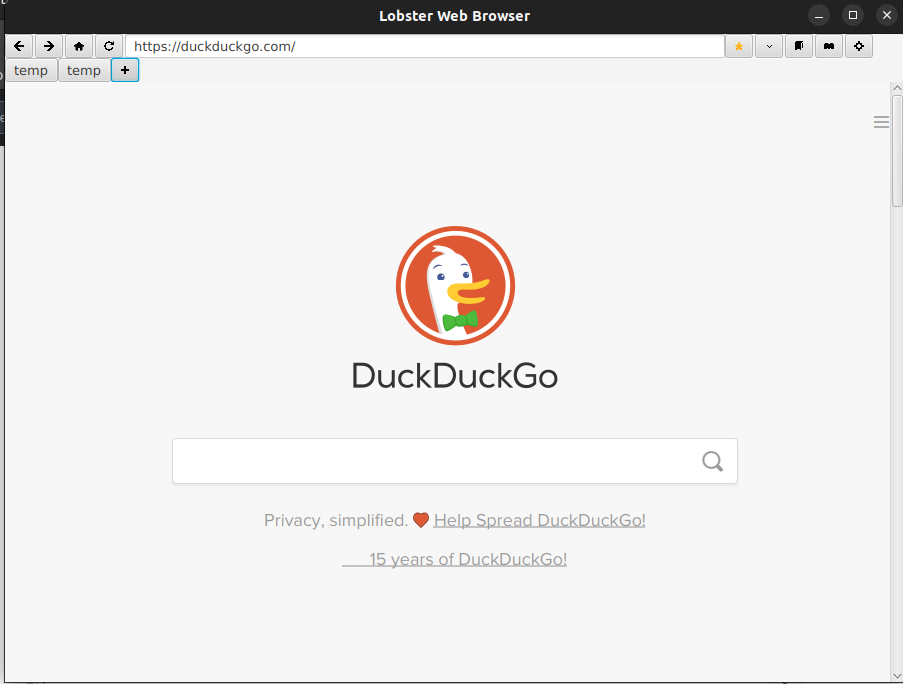
\includegraphics[width=80mm]{images/addTab.png} \par
	\normalsize \noindent By clicking on the add tab button (see selected). You can add a new tab. New tabs are added to the right of all of the previous tabs. \par
	
	
	\LARGE \noindent \justifying \textbf{Load tab:} \par
	\noindent 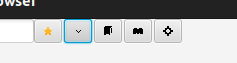
\includegraphics[height=20mm]{images/loadTab.png}
	\noindent 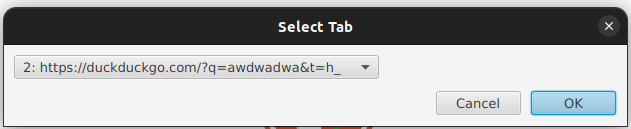
\includegraphics[height=20mm]{images/loadTabAlert.png} \par
	\normalsize \noindent By clicking on the load tab button (see selected). You switch to the selected tab. Clicking on the load tab button opens the load tab alert which has a dropdown menu that allows the user to select a tab to switch to. If the user then clicks ok with a tab selected, they will switch to that tab. If the user clicks cancel or does not select a tab then nothing will happen. \par
	
	
	\LARGE \noindent \justifying \textbf{Home button:} \par
	\noindent 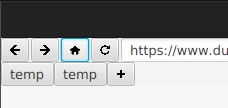
\includegraphics[width=80mm]{images/home.png} \par
	\normalsize \noindent By clicking on the home button (see selected). You can go to the home page. This will make the current tab load the homepage. No other tabs are affected. \par
	
	
	\LARGE \noindent \justifying \textbf{Forward button:} \par
	\noindent 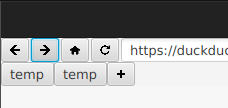
\includegraphics[width=80mm]{images/forward.png} \par
	\normalsize \noindent By clicking on the forward button (see selected). You can go to the next page in the current tab’s history. This will only change the current tab. No other tabs are affected. If there is no next page in the current tab’s history, then nothing will happen. \par
	
	\pagebreak
	
	\LARGE \noindent \justifying \textbf{Back button:} \par
	\noindent 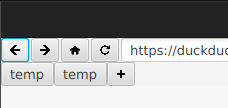
\includegraphics[width=80mm]{images/back.png} \par
	\normalsize \noindent By clicking on the back button (see selected). You can go to the previous page in the current tab’s history. This will only change the current tab. No other tabs are affected. If there is no previous page in the current tab’s history, then nothing will happen. \par
	
	
	\LARGE \noindent \justifying \textbf{Reload button:} \par
	\noindent 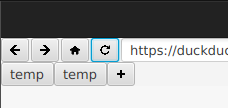
\includegraphics[width=80mm]{images/reload.png} \par
	\normalsize \noindent By clicking on the reload button (see selected). You will reload the current tab. This will only change the current tab. No other tabs are affected. \par
	
	
	\LARGE \noindent \justifying \textbf{Navigation bar:} \par
	\noindent 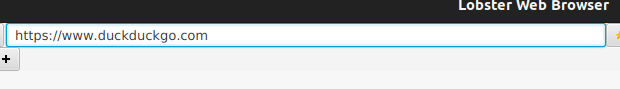
\includegraphics[width=80mm]{images/url.png} \par
	\normalsize \noindent By typing a string into the url bar then pressing enter (in the same way you would for a normal brower) you can load a webpage. If the string starts with “http”, or “www.” then it will be loaded as a url, otherwise it will be loaded as a search using duckduckgo. Url strings are edited to they always start with https:/ (if it starts with http:, https:, or http:/ then that gets replaced. If it starts with www. Then https:/ gets added to the start.). Any special characters in search strings get encoded, so they can become part of the search url.
	Note: if the user types “!@\#\$\%\textsuperscript{$\wedge$}\&*()” into the search bar (excludes the quotation marks), then they will get redirected to twitter.com. This is a feature of duckduckgo search. \par
	 
	 
	 \LARGE \noindent \justifying \textbf{Add Bookmark:} \par
	 \noindent 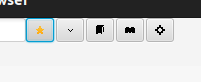
\includegraphics[height=20mm]{images/addBookmark.png}
	 \noindent 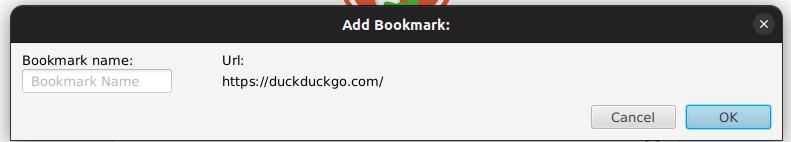
\includegraphics[height=20mm]{images/addBookmarkAlert.png} \par
	 \normalsize \noindent By clicking on the add bookmark button (see selected). You can add the current url of the current tab as a bookmark. Bookmarks are saved in a text file in the misc folder. If this folder is not there, you will not be able to add or load bookmarks. Clicking on the button creates the alert shown above. The user can edit the name of the bookmark in the appropriate text field. If the user clicks the cancel button, the bookmark will not be added. If ther user leaves the name field blank (or fills it with just spaces) then another alert will show up (see below). Dismissing that alert brings the user back to the add bookmark alert. \par
	 \noindent 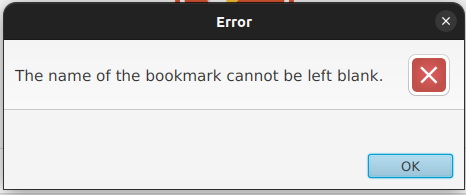
\includegraphics[width=80mm]{images/blankNameBookmark.png} \par
	 
	 	\pagebreak
	 
	 \LARGE \noindent \justifying \textbf{Load Bookmark:} \par
	 \noindent 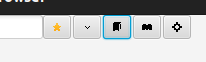
\includegraphics[height=20mm]{images/loadBookmark.png}
	 \noindent 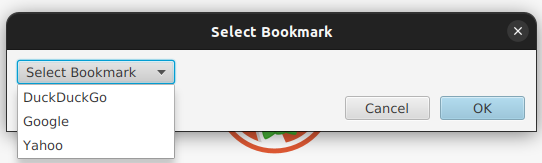
\includegraphics[height=20mm]{images/loadBookmarkAlert.png} \par
	 \normalsize \noindent By clicking on the load bookmark button (see selected). You can load one of the saved bookmarks into the current tab. Clicking on the load button loads the load bookmark alert which has a dropdown menu that allows the user to select a bookmark to load. If the user then clicks ok with a bookmark selected, then that bookmark will be loaded. If the user clicks cancel or does not select a bookmark then nothing will happen. \par
	 
	 
	 \LARGE \noindent \justifying \textbf{Change Settings:} \par
	 \noindent 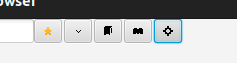
\includegraphics[height=20mm]{images/settings.png}
	 \noindent 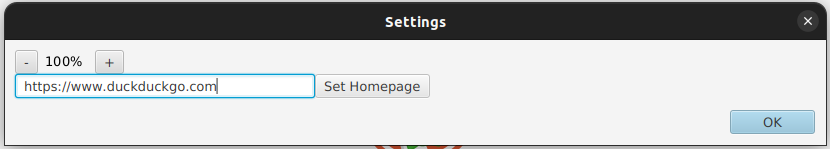
\includegraphics[height=20mm]{images/settingsAlert.png} \par
	 \normalsize \noindent By clicking on the settings button (see selected). You can change the settings. There are only 2 settings: zoom and home page. Clicking on the settings button loads the settings bookmark alert has  a text field that allows the user to enter a url and a button to set the homepage to that url (note: this homepage is for this session only). The settings alert also has a zoom in (+ symbol) button and zoom out (- symbol) button that allows the user to zoom in and zoom out. The current zoom (in \%) is also displayed as text between these buttons. The zoom is the same for all tabs (including newly created tabs). The values for the zoom range between 30\% and 500\%, these values are the same as the zoom values for firefox. If the user tries to zoom out when the zoom is at 30\% or tries to zoom in when the zoom is at 500\%, nothing will happen. \par
	 
	 
	 \LARGE \noindent \justifying \textbf{Load History} \par
	 \noindent 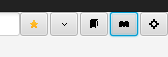
\includegraphics[height=20mm]{images/history.png}
	 \noindent 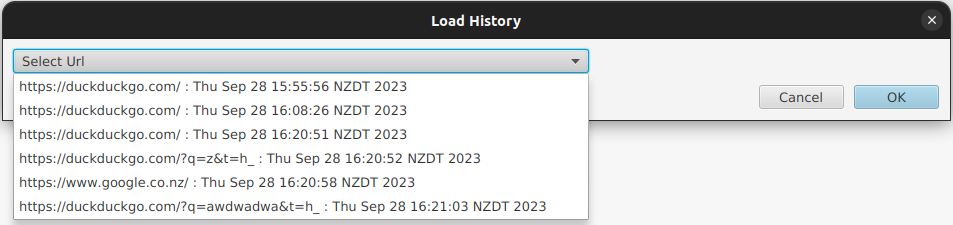
\includegraphics[height=20mm]{images/historyAlert.png} \par
	 \normalsize \noindent By clicking on the load history button (see selected). You can load a webpage save in the history into the current tab. Clicking on the load history button loads the load history alert which has a dropdown menu that allows the user to select a url to load. If the user then clicks ok with a url selected, then that url will be loaded. If the user clicks cancel or does not select a url then nothing will happen. \par
	 
	 
	 \LARGE \noindent \justifying \textbf{History} \par
	 \normalsize \noindent The history itself is a ModifiableObservableList that holds HistoryItem objects. Each tab has a WebHistory with a listener that will add new HistoryItems whenever they change webpage. These listeners also change the url in the navigation bar to the url of that webpage.
	 HistoryItem objects hold two fields: historyEntry (a WebHistory.Entry object) and its url. The HistoryItem class was created so I could change the toString method so the load history combo box would look nicer. Note: there is an issue with the date of a WebHistory.Entry object where its Date field would be null and this field is used in HistoryItem’s toString method. To avoid this issue the date used will be the current time. \par
\end{document}